\documentclass[10pt,a4paper,titlepage]{article}

\usepackage[english]{babel}
\usepackage[T1]{fontenc}
\usepackage[utf8x]{inputenc}
\usepackage[a4paper,includeheadfoot,dvipdfm,pdftex]{geometry}
\usepackage{pslatex}
\usepackage{booktabs}
\usepackage{longtable}
\usepackage{multicol}
\usepackage{tabularx}
\usepackage{fancyhdr}
\usepackage{ifthen}
\usepackage[table]{xcolor}
\usepackage[htt]{hyphenat}
\usepackage{tikz}
\usepackage{pgfplots}
\usepackage{hyperref}
\hypersetup{
    breaklinks = true,
    colorlinks = true,
    urlcolor   = blue,
    citecolor  = black,
    filecolor  = black,
    linkcolor  = black
}
\geometry{
    top      = 20mm,
    left     = 20mm,
    right    = 20mm,
    bottom   = 50mm,
    headsep  = 10mm,
    footskip = 10mm
}
\setlength{\parindent}{0cm}

\pagestyle{fancy}
\fancyhfoffset[R]{0mm}

\voffset-10mm
\topmargin0mm
\headsep10mm
\headheight20mm
\hbadness=10000
\vbadness=10000

\usepackage{caption}
\captionsetup{
   labelfont = bf,
   textfont  = it,
}

\newif\ifcopyright
\copyrightfalse % \copyrighttrue for copyright, \copyrightfalse for no copyright

\newif\ifwatermark
\watermarkfalse % \watermarktrue for watermark, \watermarkfalse for no watermark

\newif\iflogaxis
\logaxistrue % \logaxistrue for logarithmic scale, \logaxisfalse for "normal" scale

\iflogaxis
    \def\loglabel{ [log]}
\else
    \def\loglabel{}
\fi

\fancyhf{}
\renewcommand{\headrulewidth}{0pt}

\ifcopyright
    \newcommand{\mycopyright}{%
        {\small Copyright \copyright\ __COPYRIGHT__}%
    }
    % Copyright on the title page
    \fancypagestyle{empty}{\cfoot{\mycopyright}}
\fi

\cfoot{%
    {\bf\thepage}\\%
    \ifcopyright
        \mycopyright
    \fi
}

\ifwatermark
    \usepackage{draftwatermark}
    \SetWatermarkText{__WATERMARK__}
    \SetWatermarkLightness{0.9}
\fi

\newcommand{\HRule}[1]{\rule{\linewidth}{#1}}

\newcolumntype{N}{>{\raggedright\arraybackslash}m{0.5\textwidth}}
\newcolumntype{O}{>{\raggedleft\arraybackslash}m{0.2\textwidth}}
\newcolumntype{R}{>{\raggedleft\arraybackslash}X}
\newcolumntype{L}{>{\raggedright\arraybackslash}X}

% New page for each section
\let\stdsection\section
\renewcommand\section{\clearpage\stdsection}

% Alternate row color
\newcommand\altrowcolorodd{__TABLE_ODD_COLOR__}
\newcommand\altrowcoloreven{__TABLE_EVEN_COLOR__}

% Fill in color for charts
\newcommand\chartcolor{__CHART_COLOR__}

% pgfplots configuration
\pgfset{
    bar width = 14pt,
}

\pgfplotsset{
    compat = newest,
    width = \textwidth,
    height = 0.3\textheight,
    x tick label style = {/pgf/number format/1000 sep=},
    legend style = {
        at = { (0.5, -0.15) },
        anchor = north,
        legend columns = -1
    },
    ybar,
    xtick = data,
    point meta = rawy,
    axis on top,
    axis x line* = bottom,
    axis y line* = left,
    y axis line style = {opacity=0},
    yticklabels = {\empty},
    ytick style = {draw=none},
    enlarge y limits = {upper, value=0.11},
    nodes near coords,
    nodes near coords align = {vertical},
}

\iflogaxis
\pgfplotsset{ymin = 1}
\else
\pgfplotsset{ymin = 0}
\fi

% longtable
\let\oldlongtable\longtable
\let\endoldlongtable\endlongtable
\renewenvironment{longtable}{%
    \rowcolors{2}{\altrowcoloreven}{\altrowcolorodd}%
    \oldlongtable%
}{%
    \endoldlongtable%
    \global\rownum=0\relax%
}
% tabular
\let\oldtabular\tabular
\let\endoldtabular\endtabular
\renewenvironment{tabular}{%
    \rowcolors{2}{\altrowcoloreven}{\altrowcolorodd}%
    \oldtabular%
}{%
    \endoldtabular%
    \global\rownum=0\relax%
}
% tabularx
\let\oldtabularx\tabularx
\let\endoldtabularx\endtabularx
\renewenvironment{tabularx}{%
    \rowcolors{2}{\altrowcoloreven}{\altrowcolorodd}%
    \oldtabularx%
}{%
    \endoldtabularx%
    \global\rownum=0\relax%
}

\title{%
    \HRule{0.5pt}\\[0.2cm]
    \Huge\textbf{__TITLE__}\\[0.2cm]
    %__BEGIN_FILE_REQUIRED__
    \Large\texttt{__FILENAME__}\\
    %__END_FILE_REQUIRED__
    %__BEGIN_DB_REQUIRED__
    \Large __DBTYPE__ database\\
    \texttt{__FILENAME__}\\[0.2cm]
    \large __PERIOD__
    %__END_DB_REQUIRED__
    %__BEGIN_NFDUMP_REQUIRED__
    \Large NetFlow\\
    \texttt{__FILENAME__}\\[0.2cm]
    \large __PERIOD__
    %__END_NFDUMP_REQUIRED__
    \HRule{2pt}\\[3.0cm]
    %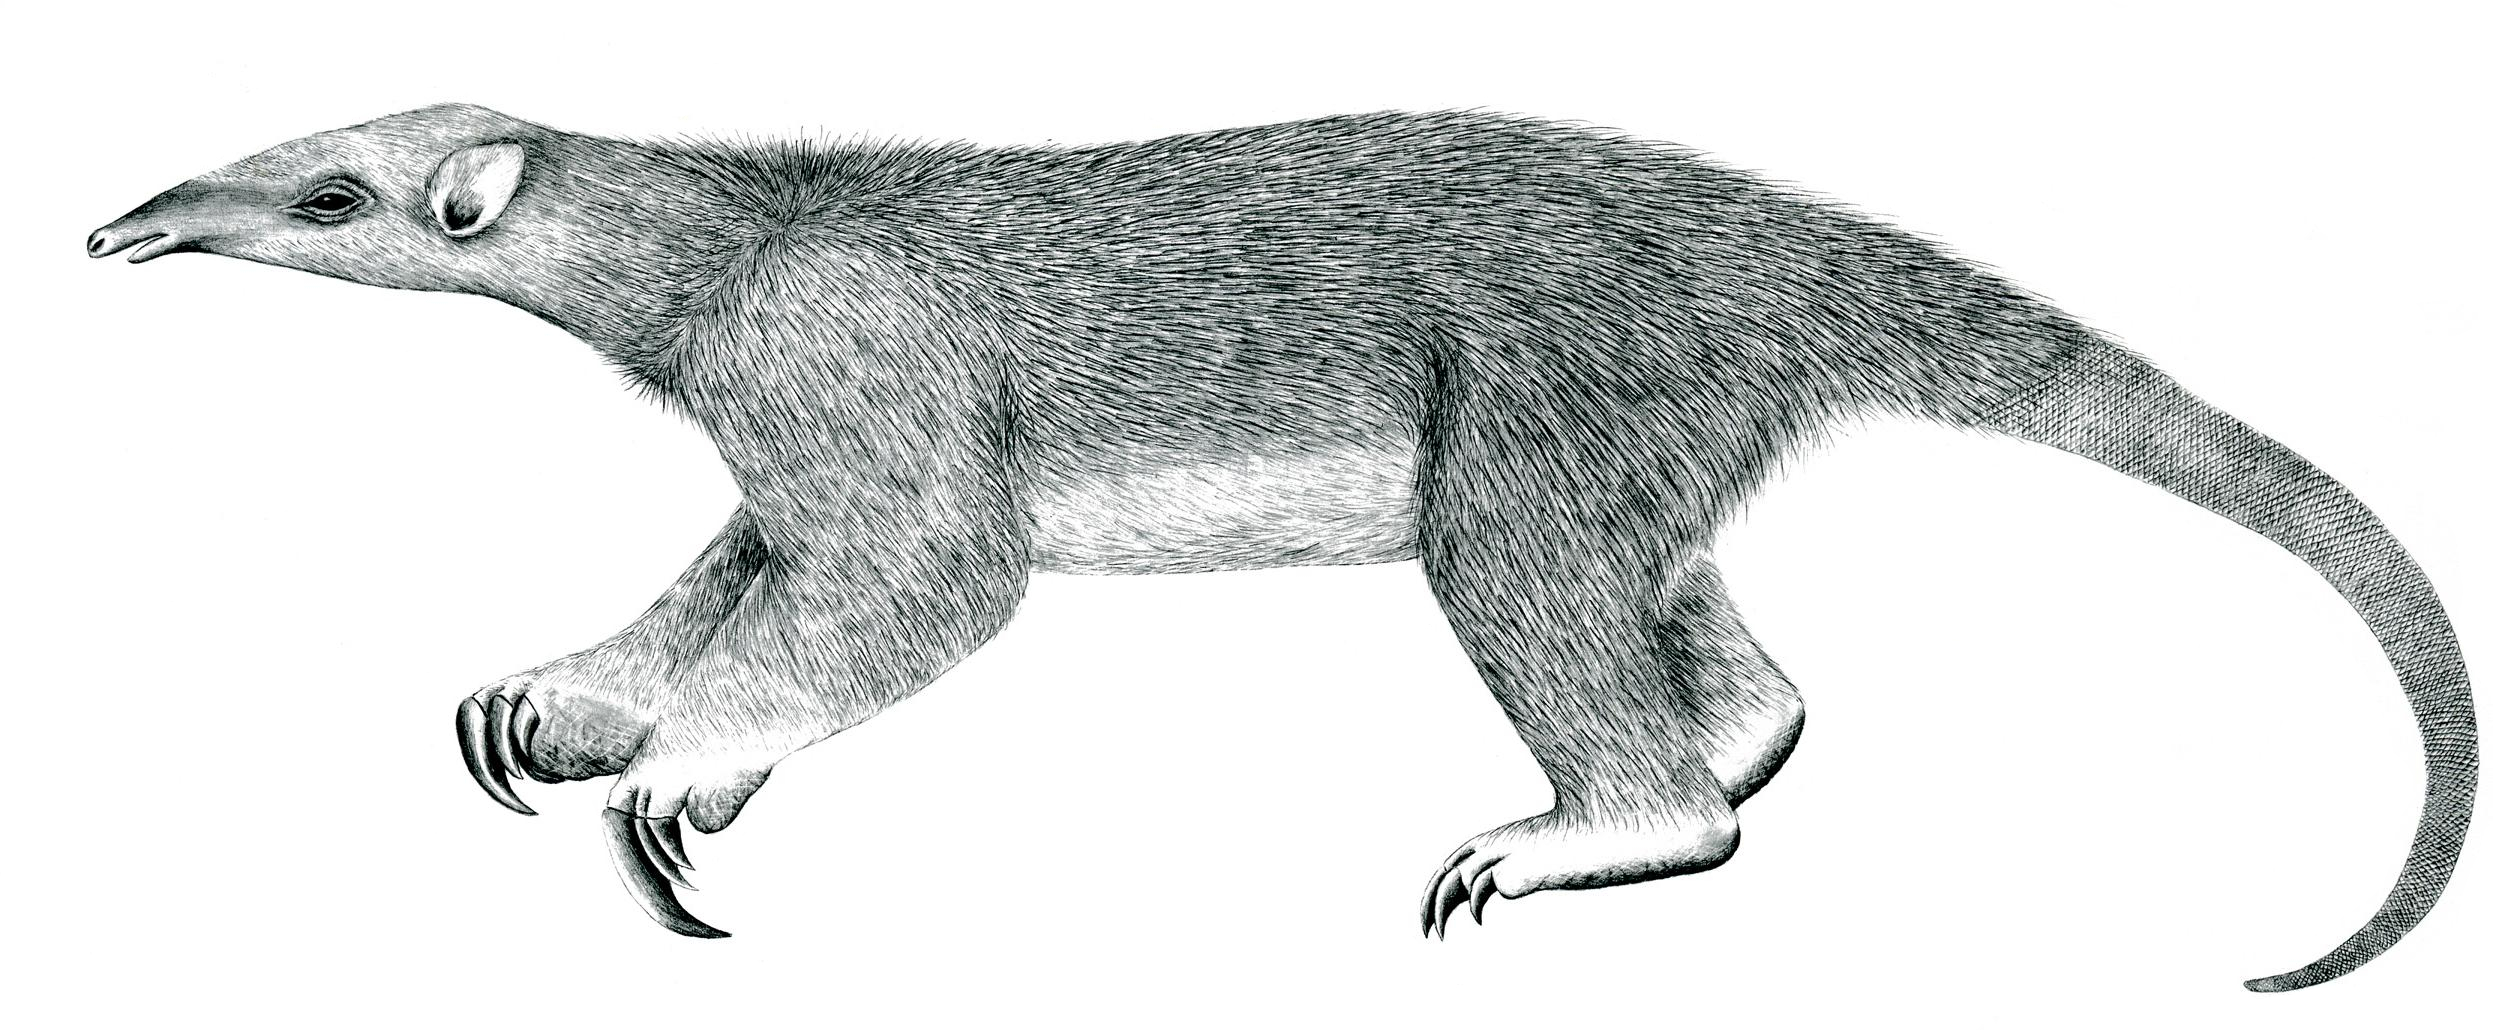
\includegraphics[scale=1.4]{img/anteater.jpg}\\
}
\author{__AUTHOR__}

\begin{document}

%\tracingall

\pagenumbering{alph}

\maketitle

\tableofcontents

\pagenumbering{arabic}

\section{Summary}
    \begin{itemize}
        %__BEGIN_FILE_REQUIRED__
        \item Filename: {\tt __FULLNAME__}
        \item MD5: {\tt __MD5SUM__}
        \item File size: __FILESIZE__
        \item Snapshot length: __SNAPLEN__
        %__END_FILE_REQUIRED__
        %__BEGIN_DB_REQUIRED__
        \item __DBTYPE__ database: {\tt __FULLNAME__}
        %__END_DB_REQUIRED__
        %__BEGIN_NFDUMP_REQUIRED__
        \item Input: {\tt __FULLNAME__}
        \item Number of input files: __NUMFILES__
        %__END_NFDUMP_REQUIRED__
        \item Number of flows: __NUMFLOWS__
        \item Number of packets: __NUMPKTS__
        \item Number of bytes: __NUMBYTES__
        \item First packet seen: __FIRSTPKT__
        \item Last packet seen: __LASTPKT__
        \item Capture duration: __DURSTR__
        %%__VLANS__%%
        %__BEGIN_DISTASNS__
        \item Number of distinct ASNs: __DISTASNS__
        %__END_DISTASNS__
        \item Number of distinct IP addresses: __DISTIP__
            \begin{itemize}
                \item __PRIVIP__ private
                \item __PUBIP__ public
                \item __DISTIP4__ IPv4
                \item __DISTIP6__ IPv6
            \end{itemize}
        %\item Min/max/average flow duration:
        %\item Min/max/average packets per flow:
        %\item Min/max/average bytes per flow:
    \end{itemize}

\section{IP addresses}

    %__BEGIN_TOP_STATS__
    \subsection{Top __TABLE_N__ IP addresses}

        % Flows

        \begin{minipage}{0.45\textwidth}
            \begin{tabular}{NOO}
                \toprule
                {\bf Src.\ IP} & {\bf Country} & {\bf Flows}\\
                \midrule
                %%__top_srcIP_flows__%%
                \bottomrule
            \end{tabular}
        \end{minipage}
        \hfill
        \begin{minipage}{0.45\textwidth}
            \begin{tabular}{NOO}
                \toprule
                {\bf Dst.\ IP} & {\bf Country} & {\bf Flows}\\
                \midrule
                %%__top_dstIP_flows__%%
                \bottomrule
            \end{tabular}
        \end{minipage}

        \vspace{\belowdisplayskip}

        % Packets

        \begin{minipage}{0.45\textwidth}
            \begin{tabular}{NOO}
                \toprule
                {\bf Src.\ IP} & {\bf Country} & {\bf Packets}\\
                \midrule
                %%__top_srcIP_pkts__%%
                \bottomrule
            \end{tabular}
        \end{minipage}
        \hfill
        \begin{minipage}{0.45\textwidth}
            \begin{tabular}{NOO}
                \toprule
                {\bf Dst.\ IP} & {\bf Country} & {\bf Packets}\\
                \midrule
                %%__top_dstIP_pkts__%%
                \bottomrule
            \end{tabular}
        \end{minipage}

        \vspace{\belowdisplayskip}

        % Bytes

        \begin{minipage}{0.45\textwidth}
            \begin{tabular}{NOO}
                \toprule
                {\bf Src.\ IP} & {\bf Country} & {\bf Bytes}\\
                \midrule
                %%__top_srcIP_bytes__%%
                \bottomrule
            \end{tabular}
        \end{minipage}
        \hfill
        \begin{minipage}{0.45\textwidth}
            \begin{tabular}{NOO}
                \toprule
                {\bf Dst.\ IP} & {\bf Country} & {\bf Bytes}\\
                \midrule
                %%__top_dstIP_bytes__%%
                \bottomrule
            \end{tabular}
        \end{minipage}
    %__END_TOP_STATS__

    %__BEGIN_BOTTOM_STATS__
    \subsection{Bottom __TABLE_N__ IP addresses}

        % Flows

        \begin{minipage}{0.45\textwidth}
            \begin{tabular}{NOO}
                \toprule
                {\bf Src.\ IP} & {\bf Country} & {\bf Flows}\\
                \midrule
                %%__bottom_srcIP_flows__%%
                \bottomrule
            \end{tabular}
        \end{minipage}
        \hfill
        \begin{minipage}{0.45\textwidth}
            \begin{tabular}{NOO}
                \toprule
                {\bf Dst.\ IP} & {\bf Country} & {\bf Flows}\\
                \midrule
                %%__bottom_dstIP_flows__%%
                \bottomrule
            \end{tabular}
        \end{minipage}

        \vspace{\belowdisplayskip}

        % Packets

        \begin{minipage}{0.45\textwidth}
            \begin{tabular}{NOO}
                \toprule
                {\bf Src.\ IP} & {\bf Country} & {\bf Packets}\\
                \midrule
                %%__bottom_srcIP_pkts__%%
                \bottomrule
            \end{tabular}
        \end{minipage}
        \hfill
        \begin{minipage}{0.45\textwidth}
            \begin{tabular}{NOO}
                \toprule
                {\bf Dst.\ IP} & {\bf Country} & {\bf Packets}\\
                \midrule
                %%__bottom_dstIP_pkts__%%
                \bottomrule
            \end{tabular}
        \end{minipage}

        \vspace{\belowdisplayskip}

        % Bytes

        \begin{minipage}{0.45\textwidth}
            \begin{tabular}{NOO}
                \toprule
                {\bf Src.\ IP} & {\bf Country} & {\bf Bytes}\\
                \midrule
                %%__bottom_srcIP_bytes__%%
                \bottomrule
            \end{tabular}
        \end{minipage}
        \hfill
        \begin{minipage}{0.45\textwidth}
            \begin{tabular}{NOO}
                \toprule
                {\bf Dst.\ IP} & {\bf Country} & {\bf Bytes}\\
                \midrule
                %%__bottom_dstIP_bytes__%%
                \bottomrule
            \end{tabular}
        \end{minipage}
    %__END_BOTTOM_STATS__

%__BEGIN_ASNS__
\section{ASNs}

    %__BEGIN_TOP_STATS__
    \subsection{Top __TABLE_N__ ASNs}

        \begin{minipage}{0.45\textwidth}
            \begin{tabularx}{0.9\textwidth}{lR}
                \toprule
                {\bf Src.\ ASN} & {\bf Flows}\\
                \midrule
                %%__top_srcASN_flows__%%
                \bottomrule
            \end{tabularx}
        \end{minipage}
        \hfill
        \begin{minipage}{0.45\textwidth}
            \begin{tabularx}{0.9\textwidth}{lR}
                \toprule
                {\bf Dst.\ ASN} & {\bf Flows}\\
                \midrule
                %%__top_dstASN_flows__%%
                \bottomrule
            \end{tabularx}
        \end{minipage}

        \vspace{\belowdisplayskip}

        \begin{minipage}{0.45\textwidth}
            \begin{tabularx}{0.9\textwidth}{lR}
                \toprule
                {\bf Src.\ ASN} & {\bf Packets}\\
                \midrule
                %%__top_srcASN_pkts__%%
                \bottomrule
            \end{tabularx}
        \end{minipage}
        \hfill
        \begin{minipage}{0.45\textwidth}
            \begin{tabularx}{0.9\textwidth}{lR}
                \toprule
                {\bf Dst.\ ASN} & {\bf Packets}\\
                \midrule
                %%__top_dstASN_pkts__%%
                \bottomrule
            \end{tabularx}
        \end{minipage}

        \vspace{\belowdisplayskip}

        \begin{minipage}{0.45\textwidth}
            \begin{tabularx}{0.9\textwidth}{lR}
                \toprule
                {\bf Src.\ ASN} & {\bf Bytes}\\
                \midrule
                %%__top_srcASN_bytes__%%
                \bottomrule
            \end{tabularx}
        \end{minipage}
        \hfill
        \begin{minipage}{0.45\textwidth}
            \begin{tabularx}{0.9\textwidth}{lR}
                \toprule
                {\bf Dst.\ ASN} & {\bf Bytes}\\
                \midrule
                %%__top_dstASN_bytes__%%
                \bottomrule
            \end{tabularx}
        \end{minipage}

    \clearpage
    %__END_TOP_STATS__

    %__BEGIN_BOTTOM_STATS__
    \subsection{Bottom __TABLE_N__ ASNs}

        \begin{minipage}{0.45\textwidth}
            \begin{tabularx}{0.9\textwidth}{lR}
                \toprule
                {\bf Src.\ ASN} & {\bf Flows}\\
                \midrule
                %%__bottom_srcASN_flows__%%
                \bottomrule
            \end{tabularx}
        \end{minipage}
        \hfill
        \begin{minipage}{0.45\textwidth}
            \begin{tabularx}{0.9\textwidth}{lR}
                \toprule
                {\bf Dst.\ ASN} & {\bf Flows}\\
                \midrule
                %%__bottom_dstASN_flows__%%
                \bottomrule
            \end{tabularx}
        \end{minipage}

        \vspace{\belowdisplayskip}

        \begin{minipage}{0.45\textwidth}
            \begin{tabularx}{0.9\textwidth}{lR}
                \toprule
                {\bf Src.\ ASN} & {\bf Packets}\\
                \midrule
                %%__bottom_srcASN_pkts__%%
                \bottomrule
            \end{tabularx}
        \end{minipage}
        \hfill
        \begin{minipage}{0.45\textwidth}
            \begin{tabularx}{0.9\textwidth}{lR}
                \toprule
                {\bf Dst.\ ASN} & {\bf Packets}\\
                \midrule
                %%__bottom_dstASN_pkts__%%
                \bottomrule
            \end{tabularx}
        \end{minipage}

        \vspace{\belowdisplayskip}

        \begin{minipage}{0.45\textwidth}
            \begin{tabularx}{0.9\textwidth}{lR}
                \toprule
                {\bf Src.\ ASN} & {\bf Bytes}\\
                \midrule
                %%__bottom_srcASN_bytes__%%
                \bottomrule
            \end{tabularx}
        \end{minipage}
        \hfill
        \begin{minipage}{0.45\textwidth}
            \begin{tabularx}{0.9\textwidth}{lR}
                \toprule
                {\bf Dst.\ ASN} & {\bf Bytes}\\
                \midrule
                %%__bottom_dstASN_bytes__%%
                \bottomrule
            \end{tabularx}
        \end{minipage}
    %__END_BOTTOM_STATS__
%__END_ASNS__

%__BEGIN_COUNTRIES__
\section{Countries}

    %__BEGIN_TOP_STATS__
    \subsection{Top __TABLE_N__ countries}

        % Source countries

        \begin{minipage}{0.33\textwidth}
            \begin{tabularx}{0.9\textwidth}{lR}
                \toprule
                {\bf Src.\ country} & {\bf Flows}\\
                \midrule
                %%__top_srcCC_flows__%%
                \bottomrule
            \end{tabularx}
        \end{minipage}
        \hfill
        \begin{minipage}{0.33\textwidth}
            \begin{tabularx}{0.9\textwidth}{lR}
                \toprule
                {\bf Src.\ country} & {\bf Packets}\\
                \midrule
                %%__top_srcCC_pkts__%%
                \bottomrule
            \end{tabularx}
        \end{minipage}
        \hfill
        \begin{minipage}{0.33\textwidth}
            \begin{tabularx}{0.9\textwidth}{lR}
                \toprule
                {\bf Src.\ country} & {\bf Bytes}\\
                \midrule
                %%__top_srcCC_bytes__%%
                \bottomrule
            \end{tabularx}
        \end{minipage}

        \vspace{\belowdisplayskip}

        % Destination countries

        \begin{minipage}{0.33\textwidth}
            \begin{tabularx}{0.9\textwidth}{lR}
                \toprule
                {\bf Dst.\ country} & {\bf Flows}\\
                \midrule
                %%__top_dstCC_flows__%%
                \bottomrule
            \end{tabularx}
        \end{minipage}
        \hfill
        \begin{minipage}{0.33\textwidth}
            \begin{tabularx}{0.9\textwidth}{lR}
                \toprule
                {\bf Dst.\ country} & {\bf Packets}\\
                \midrule
                %%__top_dstCC_pkts__%%
                \bottomrule
            \end{tabularx}
        \end{minipage}
        \hfill
        \begin{minipage}{0.33\textwidth}
            \begin{tabularx}{0.9\textwidth}{lR}
                \toprule
                {\bf Dst.\ country} & {\bf Bytes}\\
                \midrule
                %%__top_dstCC_bytes__%%
                \bottomrule
            \end{tabularx}
        \end{minipage}

    \clearpage
    %__END_TOP_STATS__

    %__BEGIN_BOTTOM_STATS__
    \subsection{Bottom __TABLE_N__ countries}

        % Source countries

        \begin{minipage}{0.33\textwidth}
            \begin{tabularx}{0.9\textwidth}{lR}
                \toprule
                {\bf Src.\ country} & {\bf Flows}\\
                \midrule
                %%__bottom_srcCC_flows__%%
                \bottomrule
            \end{tabularx}
        \end{minipage}
        \hfill
        \begin{minipage}{0.33\textwidth}
            \begin{tabularx}{0.9\textwidth}{lR}
                \toprule
                {\bf Src.\ country} & {\bf Packets}\\
                \midrule
                %%__bottom_srcCC_pkts__%%
                \bottomrule
            \end{tabularx}
        \end{minipage}
        \hfill
        \begin{minipage}{0.33\textwidth}
            \begin{tabularx}{0.9\textwidth}{lR}
                \toprule
                {\bf Src.\ country} & {\bf Bytes}\\
                \midrule
                %%__bottom_srcCC_bytes__%%
                \bottomrule
            \end{tabularx}
        \end{minipage}

        \vspace{\belowdisplayskip}

        % Destination countries

        \begin{minipage}{0.33\textwidth}
            \begin{tabularx}{0.9\textwidth}{lR}
                \toprule
                {\bf Dst.\ country} & {\bf Flows}\\
                \midrule
                %%__bottom_dstCC_flows__%%
                \bottomrule
            \end{tabularx}
        \end{minipage}
        \hfill
        \begin{minipage}{0.33\textwidth}
            \begin{tabularx}{0.9\textwidth}{lR}
                \toprule
                {\bf Dst.\ country} & {\bf Packets}\\
                \midrule
                %%__bottom_dstCC_pkts__%%
                \bottomrule
            \end{tabularx}
        \end{minipage}
        \hfill
        \begin{minipage}{0.33\textwidth}
            \begin{tabularx}{0.9\textwidth}{lR}
                \toprule
                {\bf Dst.\ country} & {\bf Bytes}\\
                \midrule
                %%__bottom_dstCC_bytes__%%
                \bottomrule
            \end{tabularx}
        \end{minipage}
    %__END_BOTTOM_STATS__
%__END_COUNTRIES__

%__BEGIN_ORGANIZATIONS__
\section{Organizations}

    %__BEGIN_TOP_STATS__
    \subsection{Top __TABLE_N__ organizations}

        % Flows

        \begin{minipage}{0.45\textwidth}
            \begin{center}
                \begin{tabularx}{\textwidth}{Lr}
                    \toprule
                    {\bf Src.\ org} & {\bf Flows}\\
                    \midrule
                    %%__top_srcOrg_flows__%%
                    \bottomrule
                \end{tabularx}
            \end{center}
        \end{minipage}
        \hfill
        \begin{minipage}{0.45\textwidth}
            \begin{center}
                \begin{tabularx}{\textwidth}{Lr}
                    \toprule
                    {\bf Dst.\ org} & {\bf Flows}\\
                    \midrule
                    %%__top_dstOrg_flows__%%
                    \bottomrule
                \end{tabularx}
            \end{center}
        \end{minipage}

        \vspace{\belowdisplayskip}

        % Packets

        \begin{minipage}{0.45\textwidth}
            \begin{center}
                \begin{tabularx}{\textwidth}{Lr}
                    \toprule
                    {\bf Src.\ org} & {\bf Packets}\\
                    \midrule
                    %%__top_srcOrg_pkts__%%
                    \bottomrule
                \end{tabularx}
            \end{center}
        \end{minipage}
        \hfill
        \begin{minipage}{0.45\textwidth}
            \begin{center}
                \begin{tabularx}{\textwidth}{Lr}
                    \toprule
                    {\bf Dst.\ org} & {\bf Packets}\\
                    \midrule
                    %%__top_dstOrg_pkts__%%
                    \bottomrule
                \end{tabularx}
            \end{center}
        \end{minipage}

        \vspace{\belowdisplayskip}

        % Bytes

        \begin{minipage}{0.45\textwidth}
            \begin{center}
                \begin{tabularx}{\textwidth}{Lr}
                    \toprule
                    {\bf Src.\ org} & {\bf Bytes}\\
                    \midrule
                    %%__top_srcOrg_bytes__%%
                    \bottomrule
                \end{tabularx}
            \end{center}
        \end{minipage}
        \hfill
        \begin{minipage}{0.45\textwidth}
            \begin{center}
                \begin{tabularx}{\textwidth}{Lr}
                    \toprule
                    {\bf Dst.\ org} & {\bf Bytes}\\
                    \midrule
                    %%__top_dstOrg_bytes__%%
                    \bottomrule
                \end{tabularx}
            \end{center}
        \end{minipage}
    %__END_TOP_STATS__

    %__BEGIN_BOTTOM_STATS__
    \subsection{Bottom __TABLE_N__ organizations}

        % Flows

        \begin{minipage}{0.45\textwidth}
            \begin{center}
                \begin{tabularx}{\textwidth}{Lr}
                    \toprule
                    {\bf Src.\ org} & {\bf Flows}\\
                    \midrule
                    %%__bottom_srcOrg_flows__%%
                    \bottomrule
                \end{tabularx}
            \end{center}
        \end{minipage}
        \hfill
        \begin{minipage}{0.45\textwidth}
            \begin{center}
                \begin{tabularx}{\textwidth}{Lr}
                    \toprule
                    {\bf Dst.\ org} & {\bf Flows}\\
                    \midrule
                    %%__bottom_dstOrg_flows__%%
                    \bottomrule
                \end{tabularx}
            \end{center}
        \end{minipage}

        \vspace{\belowdisplayskip}

        % Packets

        \begin{minipage}{0.45\textwidth}
            \begin{center}
                \begin{tabularx}{\textwidth}{Lr}
                    \toprule
                    {\bf Src.\ org} & {\bf Packets}\\
                    \midrule
                    %%__bottom_srcOrg_pkts__%%
                    \bottomrule
                \end{tabularx}
            \end{center}
        \end{minipage}
        \hfill
        \begin{minipage}{0.45\textwidth}
            \begin{center}
                \begin{tabularx}{\textwidth}{Lr}
                    \toprule
                    {\bf Dst.\ org} & {\bf Packets}\\
                    \midrule
                    %%__bottom_dstOrg_pkts__%%
                    \bottomrule
                \end{tabularx}
            \end{center}
        \end{minipage}

        \vspace{\belowdisplayskip}

        % Bytes

        \begin{minipage}{0.45\textwidth}
            \begin{center}
                \begin{tabularx}{\textwidth}{Lr}
                    \toprule
                    {\bf Src.\ org} & {\bf Bytes}\\
                    \midrule
                    %%__bottom_srcOrg_bytes__%%
                    \bottomrule
                \end{tabularx}
            \end{center}
        \end{minipage}
        \hfill
        \begin{minipage}{0.45\textwidth}
            \begin{center}
                \begin{tabularx}{\textwidth}{Lr}
                    \toprule
                    {\bf Dst.\ org} & {\bf Bytes}\\
                    \midrule
                    %%__bottom_dstOrg_bytes__%%
                    \bottomrule
                \end{tabularx}
            \end{center}
        \end{minipage}
    %__END_BOTTOM_STATS__
%__END_ORGANIZATIONS__

\section{Protocols}

    % Flows

    %__BEGIN_TOP_BOTTOM_STATS__
    \begin{minipage}{0.48\textwidth}
    %__END_TOP_BOTTOM_STATS__
        %__BEGIN_TOP_STATS__
        \subsection{Top __TABLE_N__ protocols}
        \begin{tikzpicture}
            \iflogaxis
                \begin{semilogyaxis}[
            \else
                \begin{axis}[
            \fi
                ylabel = {\bf Flows\loglabel},
                xlabel = {\bf Protocol},
                symbolic x coords = {
                    %%__top_proto_flows__%%
                };
            \iflogaxis
                \end{semilogyaxis}
            \else
                \end{axis}
            \fi
        \end{tikzpicture}
        %__END_TOP_STATS__
    %__BEGIN_TOP_BOTTOM_STATS__
    \end{minipage}
    \hfill
    \begin{minipage}{0.48\textwidth}
    %__END_TOP_BOTTOM_STATS__
        %__BEGIN_BOTTOM_STATS__
        \subsection{Bottom __TABLE_N__ protocols}
        \begin{tikzpicture}
            \iflogaxis
                \begin{semilogyaxis}[
            \else
                \begin{axis}[
            \fi
                ylabel = {\bf Flows\loglabel},
                xlabel = {\bf Protocol},
                symbolic x coords = {
                    %%__bottom_proto_flows__%%
                };
            \iflogaxis
                \end{semilogyaxis}
            \else
                \end{axis}
            \fi
        \end{tikzpicture}

        %__END_BOTTOM_STATS__
    %__BEGIN_TOP_BOTTOM_STATS__
    \end{minipage}
    %__END_TOP_BOTTOM_STATS__

    % Packets

    %__BEGIN_TOP_BOTTOM_STATS__
    \begin{minipage}{0.48\textwidth}
    %__END_TOP_BOTTOM_STATS__
        %__BEGIN_TOP_STATS__
        \begin{tikzpicture}
            \iflogaxis
                \begin{semilogyaxis}[
            \else
                \begin{axis}[
            \fi
                ylabel = {\bf Packets\loglabel},
                xlabel = {\bf Protocol},
                symbolic x coords = {
                    %%__top_proto_pkts__%%
                };
            \iflogaxis
                \end{semilogyaxis}
            \else
                \end{axis}
            \fi
        \end{tikzpicture}
        %__END_TOP_STATS__
    %__BEGIN_TOP_BOTTOM_STATS__
    \end{minipage}
    \hfill
    \begin{minipage}{0.48\textwidth}
    %__END_TOP_BOTTOM_STATS__
        %__BEGIN_BOTTOM_STATS__
        \begin{tikzpicture}
            \iflogaxis
                \begin{semilogyaxis}[
            \else
                \begin{axis}[
            \fi
                ylabel = {\bf Packets\loglabel},
                xlabel = {\bf Protocol},
                symbolic x coords = {
                    %%__bottom_proto_pkts__%%
                };
            \iflogaxis
                \end{semilogyaxis}
            \else
                \end{axis}
            \fi
        \end{tikzpicture}
        %__END_BOTTOM_STATS__
    %__BEGIN_TOP_BOTTOM_STATS__
    \end{minipage}
    %__END_TOP_BOTTOM_STATS__

    % Bytes

    %__BEGIN_TOP_BOTTOM_STATS__
    \begin{minipage}{0.48\textwidth}
    %__END_TOP_BOTTOM_STATS__
        %__BEGIN_TOP_STATS__
        \begin{tikzpicture}
            \iflogaxis
                \begin{semilogyaxis}[
            \else
                \begin{axis}[
            \fi
                ylabel = {\bf Bytes\loglabel},
                xlabel = {\bf Protocol},
                symbolic x coords = {
                    %%__top_proto_bytes__%%
                };
            \iflogaxis
                \end{semilogyaxis}
            \else
                \end{axis}
            \fi
        \end{tikzpicture}
        %__END_TOP_STATS__
    %__BEGIN_TOP_BOTTOM_STATS__
    \end{minipage}
    \hfill
    \begin{minipage}{0.48\textwidth}
    %__END_TOP_BOTTOM_STATS__
        %__BEGIN_BOTTOM_STATS__
        \begin{tikzpicture}
            \iflogaxis
                \begin{semilogyaxis}[
            \else
                \begin{axis}[
            \fi
                ylabel = {\bf Bytes\loglabel},
                xlabel = {\bf Protocol},
                symbolic x coords = {
                    %%__bottom_proto_bytes__%%
                };
            \iflogaxis
                \end{semilogyaxis}
            \else
                \end{axis}
            \fi
        \end{tikzpicture}
        %__END_BOTTOM_STATS__
    %__BEGIN_TOP_BOTTOM_STATS__
    \end{minipage}
    %__END_TOP_BOTTOM_STATS__

\section{TCP ports}

    %__BEGIN_TOP_STATS__
    \subsection{Top __CHART_N__ TCP ports}

        % Flows

        \begin{minipage}{0.48\textwidth}
            \begin{tikzpicture}
                \iflogaxis
                    \begin{semilogyaxis}[
                \else
                    \begin{axis}[
                \fi
                    ylabel = {\bf Flows\loglabel},
                    xlabel = {\bf Destination port},
                    symbolic x coords = {
                        %%__top_tcp_dstPort_flows__%%
                    };
                \iflogaxis
                    \end{semilogyaxis}
                \else
                    \end{axis}
                \fi
            \end{tikzpicture}
        \end{minipage}
        \hfill
        \begin{minipage}{0.48\textwidth}
            \begin{tikzpicture}
                \raggedleft
                \iflogaxis
                    \begin{semilogyaxis}[
                \else
                    \begin{axis}[
                \fi
                    ylabel = {\bf Flows\loglabel},
                    xlabel = {\bf Source port},
                    symbolic x coords = {
                        %%__top_tcp_srcPort_flows__%%
                    };
                \iflogaxis
                    \end{semilogyaxis}
                \else
                    \end{axis}
                \fi
            \end{tikzpicture}
        \end{minipage}

        % Packets

        \begin{minipage}{0.48\textwidth}
            \begin{tikzpicture}
                \iflogaxis
                    \begin{semilogyaxis}[
                \else
                    \begin{axis}[
                \fi
                    ylabel = {\bf Packets\loglabel},
                    xlabel = {\bf Destination port},
                    symbolic x coords = {
                        %%__top_tcp_dstPort_pkts__%%
                    };
                \iflogaxis
                    \end{semilogyaxis}
                \else
                    \end{axis}
                \fi
            \end{tikzpicture}
        \end{minipage}
        \hfill
        \begin{minipage}{0.48\textwidth}
            \begin{tikzpicture}
                \iflogaxis
                    \begin{semilogyaxis}[
                \else
                    \begin{axis}[
                \fi
                    ylabel = {\bf Packets\loglabel},
                    xlabel = {\bf Source port},
                    symbolic x coords = {
                        %%__top_tcp_srcPort_pkts__%%
                    };
                \iflogaxis
                    \end{semilogyaxis}
                \else
                    \end{axis}
                \fi
            \end{tikzpicture}
        \end{minipage}

        % Bytes

        \begin{minipage}{0.48\textwidth}
            \begin{tikzpicture}
                \iflogaxis
                    \begin{semilogyaxis}[
                \else
                    \begin{axis}[
                \fi
                    ylabel = {\bf Bytes\loglabel},
                    xlabel = {\bf Destination port},
                    symbolic x coords = {
                        %%__top_tcp_dstPort_bytes__%%
                    };
                \iflogaxis
                    \end{semilogyaxis}
                \else
                    \end{axis}
                \fi
            \end{tikzpicture}
        \end{minipage}
        \hfill
        \begin{minipage}{0.48\textwidth}
            \begin{tikzpicture}
                \iflogaxis
                    \begin{semilogyaxis}[
                \else
                    \begin{axis}[
                \fi
                    ylabel = {\bf Bytes\loglabel},
                    xlabel = {\bf Source port},
                    symbolic x coords = {
                        %%__top_tcp_srcPort_bytes__%%
                    };
                \iflogaxis
                    \end{semilogyaxis}
                \else
                    \end{axis}
                \fi
            \end{tikzpicture}
        \end{minipage}
    %__END_TOP_STATS__

    %__BEGIN_BOTTOM_STATS__
    \subsection{Bottom __CHART_N__ TCP ports}

        % Flows

        \begin{minipage}{0.48\textwidth}
            \begin{tikzpicture}
                \iflogaxis
                    \begin{semilogyaxis}[
                \else
                    \begin{axis}[
                \fi
                    ylabel = {\bf Flows\loglabel},
                    xlabel = {\bf Destination port},
                    symbolic x coords = {
                        %%__bottom_tcp_dstPort_flows__%%
                    };
                \iflogaxis
                    \end{semilogyaxis}
                \else
                    \end{axis}
                \fi
            \end{tikzpicture}
        \end{minipage}
        \hfill
        \begin{minipage}{0.48\textwidth}
            \begin{tikzpicture}
                \raggedleft
                \iflogaxis
                    \begin{semilogyaxis}[
                \else
                    \begin{axis}[
                \fi
                    ylabel = {\bf Flows\loglabel},
                    xlabel = {\bf Source port},
                    symbolic x coords = {
                        %%__bottom_tcp_srcPort_flows__%%
                    };
                \iflogaxis
                    \end{semilogyaxis}
                \else
                    \end{axis}
                \fi
            \end{tikzpicture}
        \end{minipage}

        % Packets

        \begin{minipage}{0.48\textwidth}
            \begin{tikzpicture}
                \iflogaxis
                    \begin{semilogyaxis}[
                \else
                    \begin{axis}[
                \fi
                    ylabel = {\bf Packets\loglabel},
                    xlabel = {\bf Destination port},
                    symbolic x coords = {
                        %%__bottom_tcp_dstPort_pkts__%%
                    };
                \iflogaxis
                    \end{semilogyaxis}
                \else
                    \end{axis}
                \fi
            \end{tikzpicture}
        \end{minipage}
        \hfill
        \begin{minipage}{0.48\textwidth}
            \begin{tikzpicture}
                \iflogaxis
                    \begin{semilogyaxis}[
                \else
                    \begin{axis}[
                \fi
                    ylabel = {\bf Packets\loglabel},
                    xlabel = {\bf Source port},
                    symbolic x coords = {
                        %%__bottom_tcp_srcPort_pkts__%%
                    };
                \iflogaxis
                    \end{semilogyaxis}
                \else
                    \end{axis}
                \fi
            \end{tikzpicture}
        \end{minipage}

        % Bytes

        \begin{minipage}{0.48\textwidth}
            \begin{tikzpicture}
                \iflogaxis
                    \begin{semilogyaxis}[
                \else
                    \begin{axis}[
                \fi
                    ylabel = {\bf Bytes\loglabel},
                    xlabel = {\bf Destination port},
                    symbolic x coords = {
                        %%__bottom_tcp_dstPort_bytes__%%
                    };
                \iflogaxis
                    \end{semilogyaxis}
                \else
                    \end{axis}
                \fi
            \end{tikzpicture}
        \end{minipage}
        \hfill
        \begin{minipage}{0.48\textwidth}
            \begin{tikzpicture}
                \iflogaxis
                    \begin{semilogyaxis}[
                \else
                    \begin{axis}[
                \fi
                    ylabel = {\bf Bytes\loglabel},
                    xlabel = {\bf Source port},
                    symbolic x coords = {
                        %%__bottom_tcp_srcPort_bytes__%%
                    };
                \iflogaxis
                    \end{semilogyaxis}
                \else
                    \end{axis}
                \fi
            \end{tikzpicture}
        \end{minipage}
    %__END_BOTTOM_STATS__

\section{UDP ports}

    %__BEGIN_TOP_STATS__
    \subsection{Top __CHART_N__ UDP ports}

        % Flows

        \begin{minipage}{0.48\textwidth}
            \begin{tikzpicture}
                \iflogaxis
                    \begin{semilogyaxis}[
                \else
                    \begin{axis}[
                \fi
                    ylabel = {\bf Flows\loglabel},
                    xlabel = {\bf Destination port},
                    symbolic x coords = {
                        %%__top_udp_dstPort_flows__%%
                    };
                \iflogaxis
                    \end{semilogyaxis}
                \else
                    \end{axis}
                \fi
            \end{tikzpicture}
        \end{minipage}
        \hfill
        \begin{minipage}{0.48\textwidth}
            \begin{tikzpicture}
                \raggedleft
                \iflogaxis
                    \begin{semilogyaxis}[
                \else
                    \begin{axis}[
                \fi
                    ylabel = {\bf Flows\loglabel},
                    xlabel = {\bf Source port},
                    symbolic x coords = {
                        %%__top_udp_srcPort_flows__%%
                    };
                \iflogaxis
                    \end{semilogyaxis}
                \else
                    \end{axis}
                \fi
            \end{tikzpicture}
        \end{minipage}

        % Packets

        \begin{minipage}{0.48\textwidth}
            \begin{tikzpicture}
                \iflogaxis
                    \begin{semilogyaxis}[
                \else
                    \begin{axis}[
                \fi
                    ylabel = {\bf Packets\loglabel},
                    xlabel = {\bf Destination port},
                    symbolic x coords = {
                        %%__top_udp_dstPort_pkts__%%
                    };
                \iflogaxis
                    \end{semilogyaxis}
                \else
                    \end{axis}
                \fi
            \end{tikzpicture}
        \end{minipage}
        \hfill
        \begin{minipage}{0.48\textwidth}
            \begin{tikzpicture}
                \iflogaxis
                    \begin{semilogyaxis}[
                \else
                    \begin{axis}[
                \fi
                    ylabel = {\bf Packets\loglabel},
                    xlabel = {\bf Source port},
                    symbolic x coords = {
                        %%__top_udp_srcPort_pkts__%%
                    };
                \iflogaxis
                    \end{semilogyaxis}
                \else
                    \end{axis}
                \fi
            \end{tikzpicture}
        \end{minipage}

        % Bytes

        \begin{minipage}{0.48\textwidth}
            \begin{tikzpicture}
                \iflogaxis
                    \begin{semilogyaxis}[
                \else
                    \begin{axis}[
                \fi
                    ylabel = {\bf Bytes\loglabel},
                    xlabel = {\bf Destination port},
                    symbolic x coords = {
                        %%__top_udp_dstPort_bytes__%%
                    };
                \iflogaxis
                    \end{semilogyaxis}
                \else
                    \end{axis}
                \fi
            \end{tikzpicture}
        \end{minipage}
        \hfill
        \begin{minipage}{0.48\textwidth}
            \begin{tikzpicture}
                \iflogaxis
                    \begin{semilogyaxis}[
                \else
                    \begin{axis}[
                \fi
                    ylabel = {\bf Bytes\loglabel},
                    xlabel = {\bf Source port},
                    symbolic x coords = {
                        %%__top_udp_srcPort_bytes__%%
                    };
                \iflogaxis
                    \end{semilogyaxis}
                \else
                    \end{axis}
                \fi
            \end{tikzpicture}
        \end{minipage}
    %__END_TOP_STATS__

    %__BEGIN_BOTTOM_STATS__
    \subsection{Bottom __CHART_N__ UDP ports}

        % Flows

        \begin{minipage}{0.48\textwidth}
            \begin{tikzpicture}
                \iflogaxis
                    \begin{semilogyaxis}[
                \else
                    \begin{axis}[
                \fi
                    ylabel = {\bf Flows\loglabel},
                    xlabel = {\bf Destination port},
                    symbolic x coords = {
                        %%__bottom_udp_dstPort_flows__%%
                    };
                \iflogaxis
                    \end{semilogyaxis}
                \else
                    \end{axis}
                \fi
            \end{tikzpicture}
        \end{minipage}
        \hfill
        \begin{minipage}{0.48\textwidth}
            \begin{tikzpicture}
                \raggedleft
                \iflogaxis
                    \begin{semilogyaxis}[
                \else
                    \begin{axis}[
                \fi
                    ylabel = {\bf Flows\loglabel},
                    xlabel = {\bf Source port},
                    symbolic x coords = {
                        %%__bottom_udp_srcPort_flows__%%
                    };
                \iflogaxis
                    \end{semilogyaxis}
                \else
                    \end{axis}
                \fi
            \end{tikzpicture}
        \end{minipage}

        % Packets

        \begin{minipage}{0.48\textwidth}
            \begin{tikzpicture}
                \iflogaxis
                    \begin{semilogyaxis}[
                \else
                    \begin{axis}[
                \fi
                    ylabel = {\bf Packets\loglabel},
                    xlabel = {\bf Destination port},
                    symbolic x coords = {
                        %%__bottom_udp_dstPort_pkts__%%
                    };
                \iflogaxis
                    \end{semilogyaxis}
                \else
                    \end{axis}
                \fi
            \end{tikzpicture}
        \end{minipage}
        \hfill
        \begin{minipage}{0.48\textwidth}
            \begin{tikzpicture}
                \iflogaxis
                    \begin{semilogyaxis}[
                \else
                    \begin{axis}[
                \fi
                    ylabel = {\bf Packets\loglabel},
                    xlabel = {\bf Source port},
                    symbolic x coords = {
                        %%__bottom_udp_srcPort_pkts__%%
                    };
                \iflogaxis
                    \end{semilogyaxis}
                \else
                    \end{axis}
                \fi
            \end{tikzpicture}
        \end{minipage}

        % Bytes

        \begin{minipage}{0.48\textwidth}
            \begin{tikzpicture}
                \iflogaxis
                    \begin{semilogyaxis}[
                \else
                    \begin{axis}[
                \fi
                    ylabel = {\bf Bytes\loglabel},
                    xlabel = {\bf Destination port},
                    symbolic x coords = {
                        %%__bottom_udp_dstPort_bytes__%%
                    };
                \iflogaxis
                    \end{semilogyaxis}
                \else
                    \end{axis}
                \fi
            \end{tikzpicture}
        \end{minipage}
        \hfill
        \begin{minipage}{0.48\textwidth}
            \begin{tikzpicture}
                \iflogaxis
                    \begin{semilogyaxis}[
                \else
                    \begin{axis}[
                \fi
                    ylabel = {\bf Bytes\loglabel},
                    xlabel = {\bf Source port},
                    symbolic x coords = {
                        %%__bottom_udp_srcPort_bytes__%%
                    };
                \iflogaxis
                    \end{semilogyaxis}
                \else
                    \end{axis}
                \fi
            \end{tikzpicture}
        \end{minipage}
    %__END_BOTTOM_STATS__

%__BEGIN_NOT_NFDUMP__
\section{Applications}

    % Flows

    %__BEGIN_TOP_BOTTOM_STATS__
    \begin{minipage}{0.48\textwidth}
    %__END_TOP_BOTTOM_STATS__
        %__BEGIN_TOP_STATS__
        \subsection{Top __TABLE_N__ applications}
        \begin{center}
            \begin{tabularx}{0.8\textwidth}{lR}
                \toprule
                {\bf Application} & {\bf Flows}\\
                \midrule
                %%__top_appl_flows__%%
                \bottomrule
            \end{tabularx}
        \end{center}
        %__END_TOP_STATS__
    %__BEGIN_TOP_BOTTOM_STATS__
    \end{minipage}
    \hfill
    \begin{minipage}{0.48\textwidth}
    %__END_TOP_BOTTOM_STATS__
        %__BEGIN_BOTTOM_STATS__
        \subsection{Bottom __TABLE_N__ applications}
        \begin{center}
            \begin{tabularx}{0.8\textwidth}{lR}
                \toprule
                {\bf Application} & {\bf Flows}\\
                \midrule
                %%__bottom_appl_flows__%%
                \bottomrule
            \end{tabularx}
        \end{center}
        %__END_BOTTOM_STATS__
    %__BEGIN_TOP_BOTTOM_STATS__
    \end{minipage}
    %__END_TOP_BOTTOM_STATS__

    \vspace{\belowdisplayskip}

    % Packets

    %__BEGIN_TOP_BOTTOM_STATS__
    \begin{minipage}{0.48\textwidth}
    %__END_TOP_BOTTOM_STATS__
        %__BEGIN_TOP_STATS__
        \begin{center}
            \begin{tabularx}{0.8\textwidth}{lR}
                \toprule
                {\bf Application} & {\bf Packets}\\
                \midrule
                %%__top_appl_pkts__%%
                \bottomrule
            \end{tabularx}
        \end{center}
        %__END_TOP_STATS__
    %__BEGIN_TOP_BOTTOM_STATS__
    \end{minipage}
    \hfill
    \begin{minipage}{0.48\textwidth}
    %__END_TOP_BOTTOM_STATS__
        %__BEGIN_BOTTOM_STATS__
        \begin{center}
            \begin{tabularx}{0.8\textwidth}{lR}
                \toprule
                {\bf Application} & {\bf Packets}\\
                \midrule
                %%__bottom_appl_pkts__%%
                \bottomrule
            \end{tabularx}
        \end{center}
        %__END_BOTTOM_STATS__
    %__BEGIN_TOP_BOTTOM_STATS__
    \end{minipage}
    %__END_TOP_BOTTOM_STATS__

    \vspace{\belowdisplayskip}

    % Bytes

    %__BEGIN_TOP_BOTTOM_STATS__
    \begin{minipage}{0.48\textwidth}
    %__END_TOP_BOTTOM_STATS__
        %__BEGIN_TOP_STATS__
        \begin{center}
            \begin{tabularx}{0.8\textwidth}{lR}
                \toprule
                {\bf Application} & {\bf Bytes}\\
                \midrule
                %%__top_appl_bytes__%%
                \bottomrule
            \end{tabularx}
        \end{center}
        %__END_TOP_STATS__
    %__BEGIN_TOP_BOTTOM_STATS__
    \end{minipage}
    \hfill
    \begin{minipage}{0.48\textwidth}
    %__END_TOP_BOTTOM_STATS__
        %__BEGIN_BOTTOM_STATS__
        \begin{center}
            \begin{tabularx}{0.8\textwidth}{lR}
                \toprule
                {\bf Application} & {\bf Bytes}\\
                \midrule
                %%__bottom_appl_bytes__%%
                \bottomrule
            \end{tabularx}
        \end{center}
        %__END_BOTTOM_STATS__
    %__BEGIN_TOP_BOTTOM_STATS__
    \end{minipage}
    %__END_TOP_BOTTOM_STATS__
%__END_NOT_NFDUMP__

%__BEGIN_NON_STD_PORTS__
\section{Protocols over non-standard ports}
    %__BEGIN_NDPI_AND_PORTCLASSIFIER_REQUIRED__

    %__BEGIN_TOP_STATS__
    \subsection{Top __TABLE_N__ protocols over non-standard ports}

    \begin{longtable}{llrrr}
        \toprule
        \rowcolor{\altrowcoloreven}
        {\bf Detected} & {\bf Expected} & {\bf Bytes} & {\bf Packets} & {\bf Flows}\\
        \midrule\endhead%
        %%__top_proto_over_nonstd_ports__%%
        \bottomrule
    \end{longtable}
    %__END_TOP_STATS__

    %__BEGIN_BOTTOM_STATS__
    \subsection{Bottom __TABLE_N__ protocols over non-standard ports}

    \begin{longtable}{llrrr}
        \toprule
        \rowcolor{\altrowcoloreven}
        {\bf Detected} & {\bf Expected} & {\bf Bytes} & {\bf Packets} & {\bf Flows}\\
        \midrule\endhead%
        %%__bottom_proto_over_nonstd_ports__%%
        \bottomrule
    \end{longtable}
    %__END_BOTTOM_STATS__

    % Flows

    %\begin{center}
    %    \begin{tabularx}{0.75\textwidth}{LLr}
    %        \toprule
    %        \rowcolor{\altrowcoloreven}
    %        {\bf Detected} & {\bf Expected} & {\bf Flows}\\
    %        \midrule
    %        %%__top_proto_over_nonstd_ports_flows__%%
    %        \bottomrule
    %    \end{tabularx}
    %\end{center}

    % Packets

    %\begin{center}
    %    \begin{tabularx}{0.75\textwidth}{LLr}
    %        \toprule
    %        \rowcolor{\altrowcoloreven}
    %        {\bf Detected} & {\bf Expected} & {\bf Packets}\\
    %        \midrule
    %        %%__top_proto_over_nonstd_ports_pkts__%%
    %        \bottomrule
    %    \end{tabularx}
    %\end{center}

    % Bytes

    %\begin{center}
    %    \begin{tabularx}{0.75\textwidth}{LLr}
    %        \toprule
    %        \rowcolor{\altrowcoloreven}
    %        {\bf Detected} & {\bf Expected} & {\bf Bytes}\\
    %        \midrule
    %        %%__top_proto_over_nonstd_ports_bytes__%%
    %        \bottomrule
    %    \end{tabularx}
    %\end{center}

    %__END_NDPI_AND_PORTCLASSIFIER_REQUIRED__
%__END_NON_STD_PORTS__

%__BEGIN_PASSWORDS__
\section{Cleartext passwords}

    %__BEGIN_PWX_REQUIRED__

    %__BEGIN_TOP_STATS__
    \subsection{Top __TABLE_N__ cleartext passwords}
        %%__top_passwords__%%
    %__END_TOP_STATS__

    %__BEGIN_BOTTOM_STATS__
    \subsection{Bottom __TABLE_N__ cleartext passwords}
        %%__bottom_passwords__%%
    %__END_BOTTOM_STATS__

    %__END_PWX_REQUIRED__
%__END_PASSWORDS__

%__BEGIN_DNS__
\section{DNS}

    %__BEGIN_DNSDECODE_REQUIRED__

    \subsection{DNS queries}

    %__BEGIN_TOP_STATS__
    \subsubsection{Top __TABLE_N__ DNS queries}
        \begin{tabularx}{\textwidth}{Lr}
            \toprule
            {\bf DNS query} & {\bf Count}\\
            \midrule
            %%__top_dns_queries__%%
            \bottomrule
        \end{tabularx}
    %__END_TOP_STATS__

    %__BEGIN_BOTTOM_STATS__
    \subsubsection{Bottom __TABLE_N__ DNS queries}
        \begin{tabularx}{\textwidth}{Lr}
            \toprule
            {\bf DNS query} & {\bf Count}\\
            \midrule
            %%__bottom_dns_queries__%%
            \bottomrule
        \end{tabularx}
    %__END_BOTTOM_STATS__

    \subsection{DNS answers}

    %__BEGIN_TOP_STATS__
    \subsubsection{Top __TABLE_N__ DNS answers}
        \begin{tabularx}{\textwidth}{Lr}
            \toprule
            {\bf DNS answer} & {\bf Count}\\
            \midrule
            %%__top_dns_answers__%%
            \bottomrule
        \end{tabularx}
    %__END_TOP_STATS__

    %__BEGIN_BOTTOM_STATS__
    \subsubsection{Bottom __TABLE_N__ DNS answers}
        \begin{tabularx}{\textwidth}{Lr}
            \toprule
            {\bf DNS answer} & {\bf Count}\\
            \midrule
            %%__bottom_dns_answers__%%
            \bottomrule
        \end{tabularx}
    %__END_BOTTOM_STATS__

    \subsection{DNS IPv4/6 addresses}

    %__BEGIN_TOP_STATS__
    \subsubsection{Top __TABLE_N__ DNS IPv4/6 addresses}

        \begin{minipage}{0.45\textwidth}
            \begin{center}
                \begin{tabularx}{\textwidth}{Lr}
                    \toprule
                    {\bf DNS IPv4 address} & {\bf Count}\\
                    \midrule
                    %%__top_dns_ipv4__%%
                    \bottomrule
                \end{tabularx}
            \end{center}
        \end{minipage}
        \hfill
        \begin{minipage}{0.45\textwidth}
            \begin{center}
                \begin{tabularx}{\textwidth}{Lr}
                    \toprule
                    {\bf DNS IPv6 address} & {\bf Count}\\
                    \midrule
                    %%__top_dns_ipv6__%%
                    \bottomrule
                \end{tabularx}
            \end{center}
        \end{minipage}
    %__END_TOP_STATS__

    %__BEGIN_BOTTOM_STATS__
    \subsubsection{Bottom __TABLE_N__ DNS IPv4/6 addresses}

        \begin{minipage}{0.45\textwidth}
            \begin{center}
                \begin{tabularx}{\textwidth}{Lr}
                    \toprule
                    {\bf DNS IPv4 address} & {\bf Count}\\
                    \midrule
                    %%__bottom_dns_ipv4__%%
                    \bottomrule
                \end{tabularx}
            \end{center}
        \end{minipage}
        \hfill
        \begin{minipage}{0.45\textwidth}
            \begin{center}
                \begin{tabularx}{\textwidth}{Lr}
                    \toprule
                    {\bf DNS IPv6 address} & {\bf Count}\\
                    \midrule
                    %%__bottom_dns_ipv6__%%
                    \bottomrule
                \end{tabularx}
            \end{center}
        \end{minipage}
    %__END_BOTTOM_STATS__

    \subsection{Top-Level Domains (TLD) and Second-Level Domains (SLD)}

    %__BEGIN_TOP_STATS__
    \subsubsection{Top __TABLE_N__ Top-Level Domains (TLD) and Second-Level Domains (SLD)}
        \begin{minipage}{0.45\textwidth}
            \begin{center}
                \begin{tabularx}{\textwidth}{Lr}
                    \toprule
                    {\bf TLD} & {\bf Count}\\
                    \midrule
                    %%__top_dns_tld__%%
                    \bottomrule
                \end{tabularx}
            \end{center}
        \end{minipage}
        \hfill
        \begin{minipage}{0.45\textwidth}
            \begin{center}
                \begin{tabularx}{\textwidth}{Lr}
                    \toprule
                    {\bf SLD} & {\bf Count}\\
                    \midrule
                    %%__top_dns_sld__%%
                    \bottomrule
                \end{tabularx}
            \end{center}
        \end{minipage}
    %__END_TOP_STATS__

    %__BEGIN_BOTTOM_STATS__
    \subsubsection{Bottom __TABLE_N__ Top-Level Domains (TLD) and Second-Level Domains (SLD)}
        \begin{minipage}{0.45\textwidth}
            \begin{center}
                \begin{tabularx}{\textwidth}{Lr}
                    \toprule
                    {\bf TLD} & {\bf Count}\\
                    \midrule
                    %%__bottom_dns_tld__%%
                    \bottomrule
                \end{tabularx}
            \end{center}
        \end{minipage}
        \hfill
        \begin{minipage}{0.45\textwidth}
            \begin{center}
                \begin{tabularx}{\textwidth}{Lr}
                    \toprule
                    {\bf SLD} & {\bf Count}\\
                    \midrule
                    %%__bottom_dns_sld__%%
                    \bottomrule
                \end{tabularx}
            \end{center}
        \end{minipage}
    %__END_BOTTOM_STATS__

    %__END_DNSDECODE_REQUIRED__
%__END_DNS__

%__BEGIN_HTTP__
\section{HTTP}

    %__BEGIN_HTTPSNIFFER_REQUIRED__

    \subsection{HTTP User-Agents}

    %__BEGIN_TOP_STATS__
    \subsubsection{Top __TABLE_N__ HTTP User-Agents}

        \begin{center}
            \begin{tabularx}{\textwidth}{Lr}
                \toprule
                {\bf User-Agent} & {\bf Count}\\
                \midrule
                %%__top_http_user_agent__%%
                \bottomrule
            \end{tabularx}
        \end{center}
    %__END_TOP_STATS__

    %__BEGIN_BOTTOM_STATS__
    \subsubsection{Bottom __TABLE_N__ HTTP User-Agents}

        \begin{center}
            \begin{tabularx}{\textwidth}{Lr}
                \toprule
                {\bf User-Agent} & {\bf Count}\\
                \midrule
                %%__bottom_http_user_agent__%%
                \bottomrule
            \end{tabularx}
        \end{center}
    %__END_BOTTOM_STATS__

    \subsection{HTTP Hosts and Servers}

    %__BEGIN_TOP_STATS__
    \subsubsection{Top __TABLE_N__ HTTP Hosts and Servers}

        \begin{minipage}{0.45\textwidth}
            \begin{center}
                \begin{tabularx}{\textwidth}{Lr}
                    \toprule
                    {\bf HTTP Host} & {\bf Count}\\
                    \midrule
                    %%__top_http_host__%%
                    \bottomrule
                \end{tabularx}
            \end{center}
        \end{minipage}
        \hfill
        \begin{minipage}{0.45\textwidth}
            \begin{center}
                \begin{tabularx}{\textwidth}{Lr}
                    \toprule
                    {\bf HTTP Server} & {\bf Count}\\
                    \midrule
                    %%__top_http_server__%%
                    \bottomrule
                \end{tabularx}
            \end{center}
        \end{minipage}
    %__END_TOP_STATS__

    %__BEGIN_BOTTOM_STATS__
    \subsubsection{Bottom __TABLE_N__ HTTP Hosts and Servers}

        \begin{minipage}{0.45\textwidth}
            \begin{center}
                \begin{tabularx}{\textwidth}{Lr}
                    \toprule
                    {\bf HTTP Host} & {\bf Count}\\
                    \midrule
                    %%__bottom_http_host__%%
                    \bottomrule
                \end{tabularx}
            \end{center}
        \end{minipage}
        \hfill
        \begin{minipage}{0.45\textwidth}
            \begin{center}
                \begin{tabularx}{\textwidth}{Lr}
                    \toprule
                    {\bf HTTP Server} & {\bf Count}\\
                    \midrule
                    %%__bottom_http_server__%%
                    \bottomrule
                \end{tabularx}
            \end{center}
        \end{minipage}
    %__END_BOTTOM_STATS__

    \subsection{Content-Types}

    %__BEGIN_TOP_STATS__
    \subsubsection{Top __TABLE_N__ Content-Types}

        \begin{minipage}{0.45\textwidth}
            \begin{center}
                \begin{tabularx}{\textwidth}{Lr}
                    \toprule
                    {\bf HTTP Content-Type} & {\bf Count}\\
                    \midrule
                    %%__top_http_content_type__%%
                    \bottomrule
                \end{tabularx}
            \end{center}
        \end{minipage}
        \hfill
        \begin{minipage}{0.45\textwidth}
            \begin{center}
                \begin{tabularx}{\textwidth}{Lr}
                    \toprule
                    {\bf HTTP Content-Subtypes} & {\bf Count}\\
                    \midrule
                    %%__top_http_content_subtype__%%
                    \bottomrule
                \end{tabularx}
            \end{center}
        \end{minipage}
    %__END_TOP_STATS__

    %__BEGIN_BOTTOM_STATS__
    \subsubsection{Bottom __TABLE_N__ Content-Types}

        \begin{minipage}{0.45\textwidth}
            \begin{center}
                \begin{tabularx}{\textwidth}{Lr}
                    \toprule
                    {\bf HTTP Content-Type} & {\bf Count}\\
                    \midrule
                    %%__bottom_http_content_type__%%
                    \bottomrule
                \end{tabularx}
            \end{center}
        \end{minipage}
        \hfill
        \begin{minipage}{0.45\textwidth}
            \begin{center}
                \begin{tabularx}{\textwidth}{Lr}
                    \toprule
                    {\bf HTTP Content-Subtypes} & {\bf Count}\\
                    \midrule
                    %%__bottom_http_content_subtype__%%
                    \bottomrule
                \end{tabularx}
            \end{center}
        \end{minipage}
    %__END_BOTTOM_STATS__

    % TODO requested extensions

    \subsection{HTTP Status Codes}

    %__BEGIN_TOP_STATS__
    \subsubsection{Top __CHART_N__ HTTP Status Codes}

        \begin{center}
            \begin{tikzpicture}
                \iflogaxis
                    \begin{semilogyaxis}[
                \else
                    \begin{axis}[
                \fi
                    width  = ,  % auto
                    height = ,  % auto
                    ylabel = {\bf Count\loglabel},
                    xlabel = {\bf Status Code},
                    symbolic x coords = {
                        %%__top_http_rscode__%%
                    };
                \iflogaxis
                    \end{semilogyaxis}
                \else
                    \end{axis}
                \fi
            \end{tikzpicture}
        \end{center}
    %__END_TOP_STATS__

    %__BEGIN_BOTTOM_STATS__
    \subsubsection{Bottom __CHART_N__ HTTP Status Codes}

        \begin{center}
            \begin{tikzpicture}
                \iflogaxis
                    \begin{semilogyaxis}[
                \else
                    \begin{axis}[
                \fi
                    width  = ,  % auto
                    height = ,  % auto
                    ylabel = {\bf Count\loglabel},
                    xlabel = {\bf Status Code},
                    symbolic x coords = {
                        %%__bottom_http_rscode__%%
                    };
                \iflogaxis
                    \end{semilogyaxis}
                \else
                    \end{axis}
                \fi
            \end{tikzpicture}
        \end{center}
    %__END_BOTTOM_STATS__

    %__END_HTTPSNIFFER_REQUIRED__
%__END_HTTP__

%__BEGIN_HTTPS__
\section{HTTPS}

    %__BEGIN_SSLDECODE_REQUIRED__

    \subsection{HTTPS Server Name Indication (SNI) and Certificate Common Name (CN)}

    %__BEGIN_TOP_STATS__
    \subsubsection{Top __TABLE_N__ HTTPS Server Name Indication (SNI) and Certificate Common Name (CN)}
        \begin{minipage}{0.45\textwidth}
            \begin{center}
                \begin{tabularx}{\textwidth}{Lr}
                    \toprule
                    {\bf HTTPS SNI} & {\bf Count}\\
                    \midrule
                    %%__top_https_sni__%%
                    \bottomrule
                \end{tabularx}
            \end{center}
        \end{minipage}
        \hfill
        \begin{minipage}{0.45\textwidth}
            \begin{center}
                \begin{tabularx}{\textwidth}{Lr}
                    \toprule
                    {\bf HTTPS cert.\ CN} & {\bf Count}\\
                    \midrule
                    %%__top_https_cert_cn__%%
                    \bottomrule
                \end{tabularx}
            \end{center}
        \end{minipage}
    %__END_TOP_STATS__

    %__BEGIN_BOTTOM_STATS__
    \subsubsection{Bottom __TABLE_N__ HTTPS Server Name Indication (SNI) and Certificate Common Name (CN)}
        \begin{minipage}{0.45\textwidth}
            \begin{center}
                \begin{tabularx}{\textwidth}{Lr}
                    \toprule
                    {\bf HTTPS SNI} & {\bf Count}\\
                    \midrule
                    %%__bottom_https_sni__%%
                    \bottomrule
                \end{tabularx}
            \end{center}
        \end{minipage}
        \hfill
        \begin{minipage}{0.45\textwidth}
            \begin{center}
                \begin{tabularx}{\textwidth}{Lr}
                    \toprule
                    {\bf HTTPS cert.\ CN} & {\bf Count}\\
                    \midrule
                    %%__bottom_https_cert_cn__%%
                    \bottomrule
                \end{tabularx}
            \end{center}
        \end{minipage}
    %__END_BOTTOM_STATS__

        %\begin{center}
        %    \begin{tabularx}{\textwidth}{Lr}
        %        \toprule
        %        {\bf HTTPS Cert.\ Issuer CN} & {\bf Count}\\
        %        \midrule
        %        %%__top_https_cert_issuer__%%
        %        \bottomrule
        %    \end{tabularx}
        %\end{center}

    \clearpage

    \subsection{Blacklisted certificates}

    %__BEGIN_TOP_STATS__
    \subsubsection{Top __TABLE_N__ blacklisted certificates}

        \begin{tabularx}{\textwidth}{>{\tt}lLr}
            \toprule
            {\bf HTTPS cert.\ fingerprint} & {\bf Description} & {\bf Count}\\
            \midrule
            %%__top_https_cert_bl__%%
            \bottomrule
        \end{tabularx}
    %__END_TOP_STATS__

    %__BEGIN_BOTTOM_STATS__
    \subsubsection{Bottom __TABLE_N__ blacklisted certificates}

        \begin{tabularx}{\textwidth}{>{\tt}lLr}
            \toprule
            {\bf HTTPS cert.\ fingerprint} & {\bf Description} & {\bf Count}\\
            \midrule
            %%__bottom_https_cert_bl__%%
            \bottomrule
        \end{tabularx}
    %__END_BOTTOM_STATS__

    \clearpage

    \subsection{HTTPS JA3/JA3S fingerprints}

        \subsubsection{Known HTTPS JA3 fingerprints}

        %__BEGIN_TOP_STATS__
        \paragraph{Top __TABLE_N__ known HTTPS JA3 fingerprints}~\\

            \begin{tabularx}{\textwidth}{>{\tt}lLr}
                \toprule
                {\bf JA3 fingerprint} & {\bf Description} & {\bf Count}\\
                \midrule
                %%__top_https_ja3_known__%%
                \bottomrule
            \end{tabularx}
        %__END_TOP_STATS__

        %__BEGIN_BOTTOM_STATS__
        \paragraph{Bottom __TABLE_N__ known HTTPS JA3 fingerprints}~\\

            \begin{tabularx}{\textwidth}{>{\tt}lLr}
                \toprule
                {\bf JA3 fingerprint} & {\bf Description} & {\bf Count}\\
                \midrule
                %%__bottom_https_ja3_known__%%
                \bottomrule
            \end{tabularx}
        %__END_BOTTOM_STATS__

        \clearpage

        \subsubsection{Known HTTPS JA3S fingerprints}

        %__BEGIN_TOP_STATS__
        \paragraph{Top __TABLE_N__ known HTTPS JA3S fingerprints}~\\

            \begin{tabularx}{\textwidth}{>{\tt}lLr}
                \toprule
                {\bf JA3S fingerprint} & {\bf Description} & {\bf Count}\\
                \midrule
                %%__top_https_ja3s_known__%%
                \bottomrule
            \end{tabularx}
        %__END_TOP_STATS__

        %__BEGIN_BOTTOM_STATS__
        \paragraph{Bottom __TABLE_N__ known HTTPS JA3S fingerprints}~\\

            \begin{tabularx}{\textwidth}{>{\tt}lLr}
                \toprule
                {\bf JA3S fingerprint} & {\bf Description} & {\bf Count}\\
                \midrule
                %%__bottom_https_ja3s_known__%%
                \bottomrule
            \end{tabularx}
        %__END_BOTTOM_STATS__

        \subsubsection{Unknown HTTPS JA3/JA3S fingerprints}

        %__BEGIN_TOP_STATS__
        \paragraph{Top __TABLE_N__ unknown HTTPS JA3/JA3S fingerprints}~\\

            \begin{minipage}{0.45\textwidth}
                \begin{center}
                    \begin{tabularx}{\textwidth}{Lr}
                        \toprule
                        {\bf JA3 fingerprint} & {\bf Count}\\
                        \midrule
                        %%__top_https_ja3_unknown__%%
                        \bottomrule
                    \end{tabularx}
                \end{center}
            \end{minipage}
            \hfill
            \begin{minipage}{0.45\textwidth}
                \begin{center}
                    \begin{tabularx}{\textwidth}{Lr}
                        \toprule
                        {\bf JA3S fingerprint} & {\bf Count}\\
                        \midrule
                        %%__top_https_ja3s_unknown__%%
                        \bottomrule
                    \end{tabularx}
                \end{center}
            \end{minipage}
        %__END_TOP_STATS__

        %__BEGIN_BOTTOM_STATS__
        \paragraph{Bottom __TABLE_N__ unknown HTTPS JA3/JA3S fingerprints}~\\

            \begin{minipage}{0.45\textwidth}
                \begin{center}
                    \begin{tabularx}{\textwidth}{Lr}
                        \toprule
                        {\bf JA3 fingerprint} & {\bf Count}\\
                        \midrule
                        %%__bottom_https_ja3_unknown__%%
                        \bottomrule
                    \end{tabularx}
                \end{center}
            \end{minipage}
            \hfill
            \begin{minipage}{0.45\textwidth}
                \begin{center}
                    \begin{tabularx}{\textwidth}{Lr}
                        \toprule
                        {\bf JA3S fingerprint} & {\bf Count}\\
                        \midrule
                        %%__bottom_https_ja3s_unknown__%%
                        \bottomrule
                    \end{tabularx}
                \end{center}
            \end{minipage}
        %__END_BOTTOM_STATS__

    \clearpage

    \subsection{HTTPS JA4/JA4S fingerprints}

        \subsubsection{Known HTTPS JA4 fingerprints}

        %__BEGIN_TOP_STATS__
        \paragraph{Top __TABLE_N__ known HTTPS JA4 fingerprints}~\\

            \begin{tabularx}{\textwidth}{>{\tt}lLr}
                \toprule
                {\bf JA4 fingerprint} & {\bf Description} & {\bf Count}\\
                \midrule
                %%__top_https_ja4_known__%%
                \bottomrule
            \end{tabularx}
        %__END_TOP_STATS__

        %__BEGIN_BOTTOM_STATS__
        \paragraph{Bottom __TABLE_N__ known HTTPS JA4 fingerprints}~\\

            \begin{tabularx}{\textwidth}{>{\tt}lLr}
                \toprule
                {\bf JA4 fingerprint} & {\bf Description} & {\bf Count}\\
                \midrule
                %%__bottom_https_ja4_known__%%
                \bottomrule
            \end{tabularx}
        %__END_BOTTOM_STATS__

        \subsubsection{Known HTTPS JA4S fingerprints}

        %__BEGIN_TOP_STATS__
        \paragraph{Top __TABLE_N__ known HTTPS JA4S fingerprints}~\\

            \begin{tabularx}{\textwidth}{>{\tt}lLr}
                \toprule
                {\bf JA4S fingerprint} & {\bf Description} & {\bf Count}\\
                \midrule
                %%__top_https_ja4s_known__%%
                \bottomrule
            \end{tabularx}
        %__END_TOP_STATS__

        %__BEGIN_BOTTOM_STATS__
        \paragraph{Bottom __TABLE_N__ known HTTPS JA4S fingerprints}~\\

            \begin{tabularx}{\textwidth}{>{\tt}lLr}
                \toprule
                {\bf JA4S fingerprint} & {\bf Description} & {\bf Count}\\
                \midrule
                %%__bottom_https_ja4s_known__%%
                \bottomrule
            \end{tabularx}
        %__END_BOTTOM_STATS__

        \subsubsection{Unknown HTTPS JA4/JA4S fingerprints}

        %__BEGIN_TOP_STATS__
        \paragraph{Top __TABLE_N__ unknown HTTPS JA4/JA4S fingerprints}~\\
            \begin{minipage}{0.49\textwidth}
                \begin{center}
                    \begin{tabularx}{\textwidth}{>{\tt}Lr}
                        \toprule
                        {\bf JA4 fingerprint} & {\bf Count}\\
                        \midrule
                        %%__top_https_ja4_unknown__%%
                        \bottomrule
                    \end{tabularx}
                \end{center}
            \end{minipage}
            \hfill
            \begin{minipage}{0.45\textwidth}
                \begin{center}
                    \begin{tabularx}{\textwidth}{>{\tt}Lr}
                        \toprule
                        {\bf JA4S fingerprint} & {\bf Count}\\
                        \midrule
                        %%__top_https_ja4s_unknown__%%
                        \bottomrule
                    \end{tabularx}
                \end{center}
            \end{minipage}
        %__END_TOP_STATS__

        %__BEGIN_BOTTOM_STATS__
        \paragraph{Bottom __TABLE_N__ unknown HTTPS JA4/JA4S fingerprints}~\\
            \begin{minipage}{0.49\textwidth}
                \begin{center}
                    \begin{tabularx}{\textwidth}{>{\tt}Lr}
                        \toprule
                        {\bf JA4 fingerprint} & {\bf Count}\\
                        \midrule
                        %%__bottom_https_ja4_unknown__%%
                        \bottomrule
                    \end{tabularx}
                \end{center}
            \end{minipage}
            \hfill
            \begin{minipage}{0.45\textwidth}
                \begin{center}
                    \begin{tabularx}{\textwidth}{>{\tt}Lr}
                        \toprule
                        {\bf JA4S fingerprint} & {\bf Count}\\
                        \midrule
                        %%__bottom_https_ja4s_unknown__%%
                        \bottomrule
                    \end{tabularx}
                \end{center}
            \end{minipage}
        %__END_BOTTOM_STATS__

    %__END_SSLDECODE_REQUIRED__
%__END_HTTPS__

%TODO who got what address and when
%\section{DHCP}

%__BEGIN_SSH__
\section{SSH}

    %__BEGIN_SSHDECODE_REQUIRED__
    \subsection{Top __TABLE_N__ SSH connections}
    %%__ssh__%%

    \subsection{Known HASSH fingerprints}

    %__BEGIN_TOP_STATS__
    \subsubsection{Top __TABLE_N__ known HASSH fingerprints}

        \begin{tabularx}{\textwidth}{lLr}
            \toprule
            {\bf HASSH fingerprint} & {\bf Description} & {\bf Count}\\
            \midrule
            %%__top_hassh_known__%%
            \bottomrule
        \end{tabularx}
    %__END_TOP_STATS__

    %__BEGIN_BOTTOM_STATS__
    \subsubsection{Bottom __TABLE_N__ known HASSH fingerprints}

        \begin{tabularx}{\textwidth}{lLr}
            \toprule
            {\bf HASSH fingerprint} & {\bf Description} & {\bf Count}\\
            \midrule
            %%__bottom_hassh_known__%%
            \bottomrule
        \end{tabularx}
    %__END_BOTTOM_STATS__

    %__END_SSHDECODE_REQUIRED__
%__END_SSH__

%__BEGIN_WARNINGS__
\section{Warnings}

    %__BEGIN_DATA_CARVING__
    \subsection{EXE downloads}
    %__BEGIN_HTTPSNIFFER_REQUIRED__
    %%__top_exe_dl__%%
    %__END_HTTPSNIFFER_REQUIRED__
    %__END_DATA_CARVING__

    \subsection{ARP spoofing}
    %__BEGIN_ARPDECODE_REQUIRED__
    %%__arp_spoofing__%%
    %__END_ARPDECODE_REQUIRED__

    \subsection{DNS zone transfer}
    %__BEGIN_DNSDECODE_REQUIRED__
    %%__dns_zone_transfer__%%
    %__END_DNSDECODE_REQUIRED__

%__END_WARNINGS__

\end{document}
